\section{Grand Challenge Solution}
\label{sec:solution}

For the solution a number of data processing open source frameworks have been examined, including Apache Storm and Apache Spark Streaming. Eventually, our choice fell on Flink, an Apache Foundation top project which implements a $\lambda$-architecture. The architecture of our soultion exploits some of the Flink peculiar features, the most relevant being the possibility to have a feedback 
towards upstream operators. This characteristic can be very useful in optimizing stateful nodes using data from downstream operators. In the first query it is used to delete expired posts which cannot be among the top scorer anymore. In this way we can prevent a fast growth on memory consumption as well as having only tuples around the system that con actually affect the top score.
Having to deal with graphs, we also needed something to store the data structure and that would be accessible by all the operators in the system. We dealt with this problem using Redis (Jedis API), an in-memory key-value, NoSQL database. Its versatility permits to have various data types stored in main memory, avoiding the bottleneck given by mass storage I/O. In our solution we memorize in Redis the graph represented as an adjacency list.

\begin{figure}
	\centering
	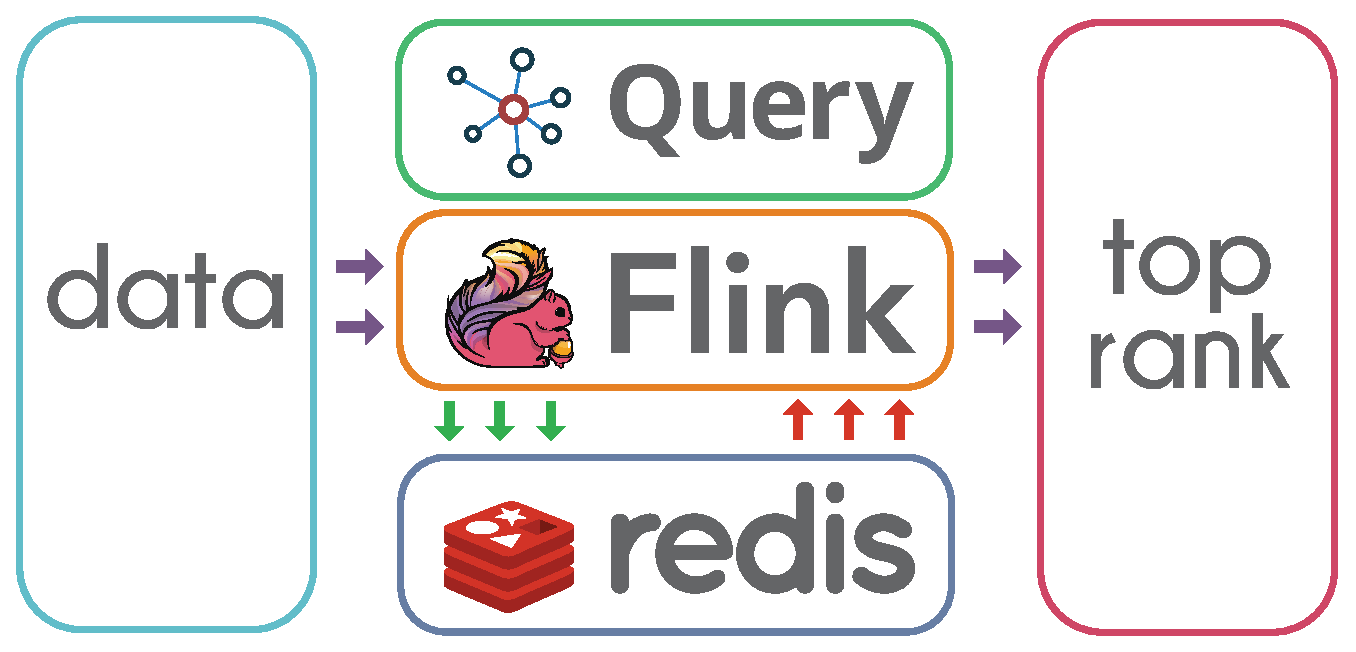
\includegraphics[width=\columnwidth]{fig/sostream-layered-architecture}
	\caption{The layered architecture}
	\label{fig:sostream-layered-architecture}
\end{figure}